\chapter{La distribution de Laplace asymétrique
  généralisée} % numéroté

Dans ce chapitre, on présente, en premier lieu, le processus de
Laplace ainsi que les deux processus sous-jacents à sa construction,
le processus gamma et le processus de Wiener. Ensuite, on présente la
distribution de Laplace asymétrique généralisée et ses principales
propriétés qui seront utilisées pour modéliser les rendements de
titres financiers. Puis, on présente quelques cas particuliers.  Dans
le chapitre suivant, on présentera différentes méthodes pour obtenir
une approximation de la fonction de densité et la fonction de
répartition.

La distribution de Laplace asymétrique généralisée a été
principalement étudiée par \cite{kozubowski1999class}. Cependant, elle
a été introduite près d'une décennie auparavant par
\cite{madan1990variance}, sous le nom de distribution Variance
Gamma. La différence entre les approches des deux auteurs est
majeure. \cite{madan1990variance} développent un modèle financier à
partir du mouvement brownien géométrique, qu'ils généralisent en
proposant que la variance suive une distribution
gamma. \cite{kozubowski1999class} généralisent la distribution de
Laplace asymétrique. Leur approche est plus générale, car ils ne
cherchent pas à développer un modèle financier, mais une nouvelle
classe de distributions utilisable dans divers domaines
scientifiques. Étant donné leur approche plus détaillée et plus
intuitive, c'est leur formulation du modèle qui sera développée. On
rappellera enfin que les deux modèles sont équivalents même si leurs
paramétrisations sont différentes.

\section{Le processus de Laplace}
\label{sec:processusGAL}

Le processus de Laplace est défini comme étant un processus de Wiener
subordonné par un processus gamma. En d'autres termes, c'est un
processus de Wiener évalué à des temps aléatoires déterminés par un
processus gamma. Selon \cite{kotz2001laplace}, ce dernier est à la
distribution de Laplace ce que le mouvement brownien est à la loi
normale. Il est aussi un cas particulier des processus de Lévy, et en
conserve donc la principale propriété, celle d'être infiniment
divisible.

Il a certains points en commun avec le mouvement brownien dont des
moments finis pour tout ordre et des incréments indépendants et
stationnaires. Cependant, la plupart des caractéristiques diffèrent:
\begin{itemize}
\item Discontinuité des trajectoires (processus de sauts);
\item Distribution asymétrique des accroissements;
\item Paramètres d'échelle et de temps entièrement dissociés.
\end{itemize}

Enfin, il possède une représentation alternative qui n'implique aucun
processus de Wiener. Il peut en fait être représenté comme la
différence de deux processus gamma indépendants. On peut le
représenter en utilisant la forme générale des processus de Lévy.

\subsection{Le processus gamma}
\label{sec:processusgamma}

Le processus gamma, noté $\left\{G(t;\tau,\beta)\right\}$, est un
processus de sauts purs (donc aucune composante de dérive ni de
diffusion) dont les incréments $G(t+1;\tau,\beta) - G(t;\tau,\beta)$
suivent une distribution gamma de paramètres de forme $\tau$ et
d'échelle $\beta$, définie par les fonctions de densité
$f_{\tau,\beta}(x)$ et caractéristique $\phi_{\tau,\beta}(\xi)$:
\begin{align}
  f_{\tau,\beta}(x) &= \frac{\beta^\tau}{\Gamma(\tau)} x^{\tau \,-\, 1} e^{- \beta x } 1_{\lbrace x\geq\,0 \rbrace} \label{eq:densitegamma} \\
  \phi_{\tau,\beta}(\xi) &= E\left[e^{i\xi\,X} \right] \nonumber\\
  &= \int_{0}^{\infty} e^{i\xi\,x} f_{\tau,\beta}(x) dx \nonumber\\
  &=
  \frac{1}{\left(1-\frac{i\xi}{\beta}\right)^{\tau}} \label{eq:fncaractgamma}.
\end{align}

On s'intéresse à la situation où le paramètre d'échelle est de valeur
unitaire ($\beta=1$). Le processus gamma agit alors à titre de
compteur et sa valeur $G(t;\tau,\beta=1)$ au temps $t$ correspondra au
nombre de sauts depuis $t=0$. La fonction de densité
$G(t+1;\tau,\beta=1) - G(t;\tau,\beta=1)$ sera alors:
\begin{align}
  f_{\tau,\beta=1}(x) &= \frac{1}{\Gamma(\tau)} x^{\tau \,-\, 1} e^{- x} 1_{\lbrace x\geq\,0 \rbrace}. \label{eq:densitegamma1}
\end{align}

Le paramètre $\tau$, qui définit la forme de la distribution,
déterminera la fréquence moyenne des sauts du processus gamma
$\Gamma(t;\tau,\beta=1)$, étant donné l'espérance $E[G(t)] = \tau\cdot
t$. La fonction caractéristique de ce processus sera donc
$\phi(\xi,t;\tau,\beta=1)$, en utilisant la propriété de convolution
\eqref{eq:convocaractIID} (même si le temps $t$ n'est pas entier, car
la distribution est infiniment divisible):
\begin{align}
  \phi(\xi,t;\tau,\beta=1) &= \left[\frac{1}{\left(1-\frac{i\xi}{1}\right)^{\tau}}\right]^t \nonumber\\
  &= \frac{1}{\left(1-i\xi\right)^{\tau\cdot t}}.
\end{align}

On peut réécrire la fonction caractéristique d'un incrément de ce
processus $\phi(\xi;t=1;\tau,\beta=1)$ sous la représentation de
Lévy-Khintchine \eqref{eq:levykhintchine}, avec l'exposant
caractéristique $\Xi(\zeta)$:
\begin{align}
  \label{eq:exposantchargamma}
  \Xi(\zeta;t=1;\tau,\beta=1) &= \tau\ln{\left(1-i\zeta\right)} \\
  &= \tau \left(e^{0} - e^{-\infty}\right) \ln{\left(1-i\zeta \right)} \nonumber\\
  &= \tau \int_{0}^{\infty} \frac{e^{-x} - e^{-(1-i\zeta)x}}{x} dx \nonumber\\
  &\qquad\mbox{(intégrale de Frullani \citep{spiegel1999schaum}, p.115)} \nonumber\\
  &= \tau \int_{0}^{\infty}
  \left(1-e^{i\zeta\,x}\right)\frac{1}{x}e^{-x}dx.
\end{align}

On a donc, par cette représentation, la démonstration que le processus
gamma est un processus de sauts purs. Il pourra donc être utilisé
comme subordonnant dans la construction d'un processus subordonné
\eqref{eq:processussubordonne}.

\subsection{Le processus de Wiener}
\label{sec:mouvementbrownien}

Le processus de Wiener $\left\{W(t;\mu,\sigma^2)\right\}$ est un
processus de diffusion avec dérive. Il n'a donc pas de composante de
saut. Ses incréments suivent une distribution normale:
\begin{align}
  \label{eq:incrwiener}
  W(t+1;\mu,\sigma^2) - W(t;\mu,\sigma^2) \sim N(\mu,\sigma^2).
\end{align}
Cette distribution est définie par la fonction de densité
$f_{\mu,\sigma}(x)$ et la fonction caractéristique
$\phi_{\mu,\sigma}(\xi)$:
\begin{align}
  f_{\mu,\sigma}(x) &= \frac{1}{\sqrt{2\pi\sigma^2}}\exp{-\left\{\frac{1}{2} \left(\frac{x-\mu}{\sigma} \right)^2\right\}} \label{eq:fndensitenormale} \\
  \phi_{\mu,\sigma}(\xi) &= \exp\left\{
    i\mu\xi-\frac{\sigma^2\xi^2}{2}
  \right\} \label{eq:fncaractnormale}.
\end{align}

Notons que la variance d'un incrément est proportionnelle à la
longueur de celui-ci.  Soit deux incréments indépendants d'un même
processus: $I_1 = W(t+q;\mu,\sigma^2) - W(t;\mu,\sigma^2) \sim
N(q\mu,q\sigma^2) \mbox{ et } I_2 = W(t+q+s;\mu,\sigma^2) -
W(t+q;\mu,\sigma^2) \sim N(s\mu,s\sigma^2)$. La somme de ces
incréments suit une distribution normale dont la moyenne et la
variance sont respectivement la somme de celles des deux incréments:
\begin{align}
  I_1+I_2 \sim N((q+s)\mu, (q+s)\sigma^2).
\end{align}

Comme la distribution normale est aussi infiniment divisible, on peut
obtenir la fonction caractéristique du processus
$\phi(\xi;t;\mu,\sigma^2)$ en utilisant la propriété de convolution
\eqref{eq:convocaractIID}:
\begin{align}
  \phi(\xi;t;\mu,\sigma^2) = \exp\left\{ i\mu t
    \xi-\frac{\sigma^2t\xi^2}{2} \right\}.
\end{align}

On déduit donc facilement l'exposant caractéristique
$\Lambda(\xi;t=1;\mu,\sigma^2)$ d'un incrément de ce processus, sous
la représentation de Lévy-Khintchine:
\begin{align}
  \label{eq:exposantcaractnormale}
  \Lambda(\xi;t=1;\mu,\sigma^2) = -(i\mu \xi-\frac{\sigma^2\xi^2}{2}).
\end{align}

Ceci démontre que le processus de Wiener est un processus avec dérive
et diffusion, mais sans composante de saut. Il pourra donc être
utilisé pour construire un processus subordonné
\eqref{eq:processussubordonne}.

\subsection{Le processus de Laplace est un processus subordonné}
\label{sec:browniensub}

On considère un processus gamma $G(t;\tau,\beta=1)$ et un processus de
Wiener $W(t;\mu,\sigma^2)$. On se rappelle que la variance d'un
incrément \eqref{eq:incrwiener} de ce dernier est proportionnelle à la
longueur de l'intervalle de temps. En utilisant une propriété appelée
la subordination, on peut modifier l'échelle de temps du processus de
Wiener de sorte que la variance soit aléatoire pour tout intervalle
. Tout processus de Lévy peut être utilisé comme subordonnant pour
définir cette échelle de temps. Si on utilise le processus gamma, on
obtiendra le processus de Laplace sans dérive
$\left\{Y(t;\sigma,\mu,\tau)\right\}$ défini comme suit:
\begin{align}
  \label{eq:VGsubordinne}
  \lbrace Y(t;\sigma,\mu,\tau)\rbrace &\equiv \lbrace
  W(G(t;\tau,\beta=1);\mu,\sigma^2)\rbrace.
\end{align}

On obtient l'exposant caractéristique $\Psi(\xi,t=1;\sigma,\mu,\tau)$
d'un incrément $Y(t+1;\sigma,\mu,\tau)-Y(t;\sigma,\mu,\tau)$ en
utilisant la propriété de subordination définie par l'équation
\eqref{eq:exposantcaractYt}, où $\Xi(\zeta,t=1;\tau,\beta=1)$ est
l'exposant caractéristique du processus gamma et
$\Lambda(\xi,t=1;\mu,\sigma^2)$ celui du processus de Wiener:
\begin{align}
  \label{eq:exposantcaractLaplace}
  \Psi(\xi,t=1;\sigma,\mu,\tau) &= \Xi(i\Lambda(\xi,t=1;\mu,\sigma^2),t=1;\tau,\beta=1) \nonumber\\
  &= \tau \ln{\left(1-i(i\Lambda(\xi)) \right)} \nonumber\\
  &= \tau \ln{\left(1+(\frac{\sigma^2 \xi^2}{2} - i \mu \xi) \right)}.
\end{align}

Le processus de Laplace sans dérive est donc, par définition, un
processus de Lévy et par conséquent infiniment divisible. En utilisant
l'exposant caractéristique \eqref{eq:exposantcaractLaplace} et la
définition \eqref{eq:fncaractYt}, on obtient sa fonction
caractéristique:
\begin{align}
  \label{eq:fonctioncaractlaplacesansdrift}
  \phi_{Y(t;\sigma,\mu,\tau)}(\xi) &= \exp{\left\{-t \cdot \Psi(\xi,t=1;\sigma,\mu,\tau)\right\}} \nonumber\\
  &= \exp{\left\{-t \cdot \left(\tau \ln{\left(1+(\frac{\sigma^2
              \xi^2}{2} - i \mu
            \xi) \right)} \right)\right\}} \nonumber\\
  &= \left(1+\frac{\sigma^2 \xi^2}{2} - i \mu \xi\right)^{-\tau \cdot
    t}.
\end{align}

Une manière simple pour expliquer le mécanisme derrière le processus
subordonné est d'en construire une trajectoire à l'aide de la
simulation.

On simule un temps d'arrivée $T_1$, de distribution gamma, puis une
hauteur de saut $X_1$, de distribution normale. On obtient ainsi le
premier incrément de la trajectoire, tel qu'illustré à la figure
\ref{fig:increment1}.
\begin{figure}[!ht]
  \centering % Graphic for TeX using PGF
% Title: /home/francois/projet-de-maitrise/graphiques/increment1.dia
% Creator: Dia v0.97.2
% CreationDate: Mon Jul 29 16:42:05 2013
% For: francois
% \usepackage{tikz}
% The following commands are not supported in PSTricks at present
% We define them conditionally, so when they are implemented,
% this pgf file will use them.
\ifx\du\undefined
  \newlength{\du}
\fi
\setlength{\du}{15\unitlength}
\begin{tikzpicture}
\pgftransformxscale{1.000000}
\pgftransformyscale{-1.000000}
\definecolor{dialinecolor}{rgb}{0.000000, 0.000000, 0.000000}
\pgfsetstrokecolor{dialinecolor}
\definecolor{dialinecolor}{rgb}{1.000000, 1.000000, 1.000000}
\pgfsetfillcolor{dialinecolor}
\pgfsetlinewidth{0.100000\du}
\pgfsetdash{}{0pt}
\pgfsetdash{}{0pt}
\pgfsetbuttcap
{
\definecolor{dialinecolor}{rgb}{0.000000, 0.000000, 0.000000}
\pgfsetfillcolor{dialinecolor}
% was here!!!
\pgfsetarrowsend{stealth}
\definecolor{dialinecolor}{rgb}{0.000000, 0.000000, 0.000000}
\pgfsetstrokecolor{dialinecolor}
\draw (19.200000\du,10.800000\du)--(28.800000\du,10.800000\du);
}
\pgfsetlinewidth{0.100000\du}
\pgfsetdash{}{0pt}
\pgfsetdash{}{0pt}
\pgfsetbuttcap
{
\definecolor{dialinecolor}{rgb}{0.000000, 0.000000, 0.000000}
\pgfsetfillcolor{dialinecolor}
% was here!!!
\pgfsetarrowsend{stealth}
\definecolor{dialinecolor}{rgb}{0.000000, 0.000000, 0.000000}
\pgfsetstrokecolor{dialinecolor}
\draw (19.200000\du,10.800000\du)--(19.200000\du,3.600000\du);
}
\pgfsetlinewidth{0.100000\du}
\pgfsetdash{}{0pt}
\pgfsetdash{}{0pt}
\pgfsetbuttcap
{
\definecolor{dialinecolor}{rgb}{0.000000, 0.000000, 0.000000}
\pgfsetfillcolor{dialinecolor}
% was here!!!
\definecolor{dialinecolor}{rgb}{0.000000, 0.000000, 0.000000}
\pgfsetstrokecolor{dialinecolor}
\draw (20.400000\du,10.600000\du)--(20.400000\du,11.000000\du);
}
\pgfsetlinewidth{0.100000\du}
\pgfsetdash{}{0pt}
\pgfsetdash{}{0pt}
\pgfsetbuttcap
{
\definecolor{dialinecolor}{rgb}{0.000000, 0.000000, 0.000000}
\pgfsetfillcolor{dialinecolor}
% was here!!!
\definecolor{dialinecolor}{rgb}{0.000000, 0.000000, 0.000000}
\pgfsetstrokecolor{dialinecolor}
\draw (26.400000\du,10.600000\du)--(26.400000\du,11.000000\du);
}
\pgfsetlinewidth{0.100000\du}
\pgfsetdash{}{0pt}
\pgfsetdash{}{0pt}
\pgfsetbuttcap
{
\definecolor{dialinecolor}{rgb}{0.000000, 0.000000, 0.000000}
\pgfsetfillcolor{dialinecolor}
% was here!!!
\definecolor{dialinecolor}{rgb}{0.000000, 0.000000, 0.000000}
\pgfsetstrokecolor{dialinecolor}
\draw (19.000000\du,9.600000\du)--(19.400000\du,9.600000\du);
}
% setfont left to latex
\definecolor{dialinecolor}{rgb}{0.000000, 0.000000, 0.000000}
\pgfsetstrokecolor{dialinecolor}
\node[anchor=west] at (20.200000\du,12.000000\du){0};
% setfont left to latex
\definecolor{dialinecolor}{rgb}{0.000000, 0.000000, 0.000000}
\pgfsetstrokecolor{dialinecolor}
\node[anchor=west] at (26.200000\du,12.000000\du){$T_1$};
% setfont left to latex
\definecolor{dialinecolor}{rgb}{0.000000, 0.000000, 0.000000}
\pgfsetstrokecolor{dialinecolor}
\node[anchor=west] at (18.200000\du,9.800000\du){0};
% setfont left to latex
\definecolor{dialinecolor}{rgb}{0.000000, 0.000000, 0.000000}
\pgfsetstrokecolor{dialinecolor}
\node[anchor=west] at (17.400000\du,6.200000\du){$X_1$};
\pgfsetlinewidth{0.100000\du}
\pgfsetdash{}{0pt}
\pgfsetdash{}{0pt}
\pgfsetbuttcap
{
\definecolor{dialinecolor}{rgb}{0.000000, 0.000000, 0.000000}
\pgfsetfillcolor{dialinecolor}
% was here!!!
\definecolor{dialinecolor}{rgb}{0.000000, 0.000000, 0.000000}
\pgfsetstrokecolor{dialinecolor}
\draw (19.000000\du,6.000000\du)--(19.400000\du,6.000000\du);
}
\pgfsetlinewidth{0.100000\du}
\pgfsetdash{}{0pt}
\pgfsetdash{}{0pt}
\pgfsetbuttcap
{
\definecolor{dialinecolor}{rgb}{0.000000, 0.000000, 0.000000}
\pgfsetfillcolor{dialinecolor}
% was here!!!
\definecolor{dialinecolor}{rgb}{0.000000, 0.000000, 0.000000}
\pgfsetstrokecolor{dialinecolor}
\draw (26.200000\du,6.000000\du)--(27.400000\du,6.000000\du);
}
\definecolor{dialinecolor}{rgb}{0.000000, 0.000000, 0.000000}
\pgfsetstrokecolor{dialinecolor}
\draw (26.200000\du,6.000000\du)--(27.400000\du,6.000000\du);
\pgfsetlinewidth{0.100000\du}
\pgfsetdash{}{0pt}
\pgfsetmiterjoin
\pgfsetbuttcap
\definecolor{dialinecolor}{rgb}{0.000000, 0.000000, 0.000000}
\pgfsetfillcolor{dialinecolor}
\pgfpathmoveto{\pgfpoint{26.200000\du}{6.000000\du}}
\pgfpathcurveto{\pgfpoint{26.200000\du}{5.875000\du}}{\pgfpoint{26.325000\du}{5.750000\du}}{\pgfpoint{26.450000\du}{5.750000\du}}
\pgfpathcurveto{\pgfpoint{26.575000\du}{5.750000\du}}{\pgfpoint{26.700000\du}{5.875000\du}}{\pgfpoint{26.700000\du}{6.000000\du}}
\pgfpathcurveto{\pgfpoint{26.700000\du}{6.125000\du}}{\pgfpoint{26.575000\du}{6.250000\du}}{\pgfpoint{26.450000\du}{6.250000\du}}
\pgfpathcurveto{\pgfpoint{26.325000\du}{6.250000\du}}{\pgfpoint{26.200000\du}{6.125000\du}}{\pgfpoint{26.200000\du}{6.000000\du}}
\pgfusepath{fill}
\definecolor{dialinecolor}{rgb}{0.000000, 0.000000, 0.000000}
\pgfsetstrokecolor{dialinecolor}
\pgfpathmoveto{\pgfpoint{26.200000\du}{6.000000\du}}
\pgfpathcurveto{\pgfpoint{26.200000\du}{5.875000\du}}{\pgfpoint{26.325000\du}{5.750000\du}}{\pgfpoint{26.450000\du}{5.750000\du}}
\pgfpathcurveto{\pgfpoint{26.575000\du}{5.750000\du}}{\pgfpoint{26.700000\du}{5.875000\du}}{\pgfpoint{26.700000\du}{6.000000\du}}
\pgfpathcurveto{\pgfpoint{26.700000\du}{6.125000\du}}{\pgfpoint{26.575000\du}{6.250000\du}}{\pgfpoint{26.450000\du}{6.250000\du}}
\pgfpathcurveto{\pgfpoint{26.325000\du}{6.250000\du}}{\pgfpoint{26.200000\du}{6.125000\du}}{\pgfpoint{26.200000\du}{6.000000\du}}
\pgfusepath{stroke}
\pgfsetlinewidth{0.100000\du}
\pgfsetdash{}{0pt}
\pgfsetdash{}{0pt}
\pgfsetbuttcap
{
\definecolor{dialinecolor}{rgb}{0.000000, 0.000000, 0.000000}
\pgfsetfillcolor{dialinecolor}
% was here!!!
}
\definecolor{dialinecolor}{rgb}{0.000000, 0.000000, 0.000000}
\pgfsetstrokecolor{dialinecolor}
\draw (20.200000\du,9.600000\du)--(26.050000\du,9.600000\du);
\pgfsetlinewidth{0.100000\du}
\pgfsetdash{}{0pt}
\pgfsetmiterjoin
\pgfsetbuttcap
\definecolor{dialinecolor}{rgb}{0.000000, 0.000000, 0.000000}
\pgfsetfillcolor{dialinecolor}
\pgfpathmoveto{\pgfpoint{20.200000\du}{9.600000\du}}
\pgfpathcurveto{\pgfpoint{20.200000\du}{9.475000\du}}{\pgfpoint{20.325000\du}{9.350000\du}}{\pgfpoint{20.450000\du}{9.350000\du}}
\pgfpathcurveto{\pgfpoint{20.575000\du}{9.350000\du}}{\pgfpoint{20.700000\du}{9.475000\du}}{\pgfpoint{20.700000\du}{9.600000\du}}
\pgfpathcurveto{\pgfpoint{20.700000\du}{9.725000\du}}{\pgfpoint{20.575000\du}{9.850000\du}}{\pgfpoint{20.450000\du}{9.850000\du}}
\pgfpathcurveto{\pgfpoint{20.325000\du}{9.850000\du}}{\pgfpoint{20.200000\du}{9.725000\du}}{\pgfpoint{20.200000\du}{9.600000\du}}
\pgfusepath{fill}
\definecolor{dialinecolor}{rgb}{0.000000, 0.000000, 0.000000}
\pgfsetstrokecolor{dialinecolor}
\pgfpathmoveto{\pgfpoint{20.200000\du}{9.600000\du}}
\pgfpathcurveto{\pgfpoint{20.200000\du}{9.475000\du}}{\pgfpoint{20.325000\du}{9.350000\du}}{\pgfpoint{20.450000\du}{9.350000\du}}
\pgfpathcurveto{\pgfpoint{20.575000\du}{9.350000\du}}{\pgfpoint{20.700000\du}{9.475000\du}}{\pgfpoint{20.700000\du}{9.600000\du}}
\pgfpathcurveto{\pgfpoint{20.700000\du}{9.725000\du}}{\pgfpoint{20.575000\du}{9.850000\du}}{\pgfpoint{20.450000\du}{9.850000\du}}
\pgfpathcurveto{\pgfpoint{20.325000\du}{9.850000\du}}{\pgfpoint{20.200000\du}{9.725000\du}}{\pgfpoint{20.200000\du}{9.600000\du}}
\pgfusepath{stroke}
\pgfsetlinewidth{0.100000\du}
\pgfsetdash{}{0pt}
\pgfsetmiterjoin
\pgfsetbuttcap
\definecolor{dialinecolor}{rgb}{1.000000, 1.000000, 1.000000}
\pgfsetfillcolor{dialinecolor}
\pgfpathmoveto{\pgfpoint{26.550000\du}{9.600000\du}}
\pgfpathcurveto{\pgfpoint{26.550000\du}{9.725000\du}}{\pgfpoint{26.425000\du}{9.850000\du}}{\pgfpoint{26.300000\du}{9.850000\du}}
\pgfpathcurveto{\pgfpoint{26.175000\du}{9.850000\du}}{\pgfpoint{26.050000\du}{9.725000\du}}{\pgfpoint{26.050000\du}{9.600000\du}}
\pgfpathcurveto{\pgfpoint{26.050000\du}{9.475000\du}}{\pgfpoint{26.175000\du}{9.350000\du}}{\pgfpoint{26.300000\du}{9.350000\du}}
\pgfpathcurveto{\pgfpoint{26.425000\du}{9.350000\du}}{\pgfpoint{26.550000\du}{9.475000\du}}{\pgfpoint{26.550000\du}{9.600000\du}}
\pgfusepath{fill}
\definecolor{dialinecolor}{rgb}{0.000000, 0.000000, 0.000000}
\pgfsetstrokecolor{dialinecolor}
\pgfpathmoveto{\pgfpoint{26.550000\du}{9.600000\du}}
\pgfpathcurveto{\pgfpoint{26.550000\du}{9.725000\du}}{\pgfpoint{26.425000\du}{9.850000\du}}{\pgfpoint{26.300000\du}{9.850000\du}}
\pgfpathcurveto{\pgfpoint{26.175000\du}{9.850000\du}}{\pgfpoint{26.050000\du}{9.725000\du}}{\pgfpoint{26.050000\du}{9.600000\du}}
\pgfpathcurveto{\pgfpoint{26.050000\du}{9.475000\du}}{\pgfpoint{26.175000\du}{9.350000\du}}{\pgfpoint{26.300000\du}{9.350000\du}}
\pgfpathcurveto{\pgfpoint{26.425000\du}{9.350000\du}}{\pgfpoint{26.550000\du}{9.475000\du}}{\pgfpoint{26.550000\du}{9.600000\du}}
\pgfusepath{stroke}
\end{tikzpicture}

  \caption{Premier incrément d'un processus subordonné}
  \label{fig:increment1}
\end{figure}

Une réalisation d'une trajectoire de ce processus par simulation se
trouve à la figure \ref{fig:simgammagauss}.

\begin{figure}[!ht]
  \centering
  \includegraphics[scale=.8]{"./graphiques/CH3-SIMGAMMAGAUSS"}
  \caption{Simulation d'un processus de Wiener subordonné par un
    processus gamma}
  \label{fig:simgammagauss}
\end{figure}

Le processus gamma $G(t;\tau,\beta=1)$, en tant que subordonnant dans
ce cas-ci, définit une échelle de temps économique , selon laquelle
on situe l'arrivée d'évènements pouvant influencer le prix d'un titre
financier. Cette dernière ne peut être mesurée, elle est donc
abstraite. L'échelle de temps où sont effectuées les observations du
processus correspond au temps calendrier. C'est la seule qui
puisse être mesurée. Étant donné que ces deux échelles sont
indépendantes, plusieurs sauts entre deux observations sont possibles.
L'échelle de temps économique est donc soit étirée, soit compressée,
en comparaison au temps calendrier. Autrement dit, si l'on définit
une journée économique comme étant l'intervalle de temps entre deux
sauts, on peut en avoir plusieurs au cours d'une seule journée de
calendrier $(G(t+1;\tau,\beta=1)-G(t;\tau,\beta=1) > 1)$. À l'opposé,
une d'entre elles peut chevaucher plusieurs journées calendrier
$(G(t+1;\tau,\beta=1)-G(t;\tau,\beta=1) \leq 1)$.

Un processus stochastique qui représente le comportement du prix d'un
titre financier doit inclure une composante de dérive.  Celle-ci
exprime le rendement moyen réalisé et est indépendante du processus de
sauts. Pour cette raison, on ajoute un coefficient de dérive $\theta$
au processus de Laplace sans dérive, pour obtenir sa forme
générale. Comme ce coefficient est constant, on peut multiplier la
fonction caractéristique \eqref{eq:fonctioncaractlaplacesansdrift} par
la transformée de Fourier inverse du produit de celui-ci et de la
longueur de l'intervalle de temps $t$, $\mathcal{F}^{-1}(\theta \cdot
t) = e^{i\xi\theta \cdot t}$, pour obtenir celle du processus de
Laplace:
\begin{align}
  \phi_{Y(t;\theta,\sigma,\mu,\tau)}(\xi) &= \frac{e^{i\xi\theta\cdot t}}{\left(1+\frac{\sigma^2\xi^2}{2}- i\mu \xi \right)^{\tau \cdot t}} \nonumber\\
  &= \left(\frac{e^{i\xi\theta}}{\left(1+\frac{\sigma^2\xi^2}{2}- i\mu
        \xi
      \right)^{\tau}}\right)^{t} \label{eq:fncaractprocessuslaplace}.
\end{align}

Le processus $\left\{Y(t;\theta,\sigma,\mu,\tau)\right\}$ définit,
dans le contexte financier, l'évolution du logarithme du prix, tel que
présenté par \cite{kotz2001laplace}. Pour des fins de simplification,
on fixe le prix initial à 1: $Y(0;\theta,\sigma,\mu,\tau) = 0$

La fonction caractéristique \eqref{eq:fncaractprocessuslaplace}
constituera la principale représentation du processus de Laplace pour
la suite de ce texte.  La construction du modèle «Variance Gamma» de
\cite{madan1990variance} est similaire, à l'exception que la
paramétrisation et le processus gamma utilisés sont différents, ce qui
rend leur approche moins intuitive, bien que le résultat soit
équivalent.

\section{Distribution de Laplace asymétrique généralisée}
\label{sec:distributionGAL}

La distribution de Laplace asymétrique généralisée caractérise un
intervalle du processus de Laplace avec dérive. Aussi appelée
distribution de Bessel, elle a été introduite par Karl Pearson en
1929, en lien avec la covariance d'un échantillon tiré d'une
population normale à deux variables. C'est aussi une généralisation de
la distribution de Laplace asymétrique qui sera présentée à la section
\ref{sec:distributionAL}.

\subsection{Fonction caractéristique}
\label{sec:fncaractGAL}

On définit cette distribution principalement par sa fonction
caractéristique. Celle-ci s'obtient facilement à partir de la fonction
caractéristique du processus de Laplace avec dérive
\eqref{eq:fncaractprocessuslaplace}, en considérant un incrément de
longueur $t=1$. À partir de la définition de ce dernier
\eqref{eq:VGsubordinne}, on déduit qu'elle est en fait un mélange de
la loi normale dont le paramètre de variance suit une distribution
gamma.

$Y$ est une variable aléatoire définie comme étant la somme:
\begin{itemize}
\item d'un paramètre de translation $\theta$,
\item du produit:
  \begin{itemize}
  \item d'une variable aléatoire $W$ issue d'une distribution gamma
    \eqref{eq:densitegamma1}
  \item et d'un paramètre $\mu$
  \end{itemize}
\item et du produit:
  \begin{itemize}
  \item d'un paramètre $\sigma$,
  \item de la racine carrée de la variable aléatoire $W$
  \item et d'une variable aléatoire $Z$ issue d'une distribution
    normale centrée réduite:
    \begin{align}
  		\label{eq:defvarY-GAL}
  		&Y = \theta + \mu W + \sigma \sqrt{W} Z
	\end{align}
	où 
	\begin{align}
  		Z \sim N(0,1) \mbox{ et } W \sim \Gamma(\tau,\beta=1). \nonumber
	\end{align}
  \end{itemize}
\end{itemize}

Alors, la variable aléatoire $Y$, sachant que $W=w$, suit une
distribution normale de moyenne $w\mu$ et de variance $w\sigma^2$:
\begin{align}
  \label{eq:Ynormalconditionnel}
  (Y|W=w) \sim N(w\mu,w\sigma^2).
\end{align}

La fonction caractéristique de la variable aléatoire $Y$ peut donc
être obtenue en utilisant celle de la loi normale $\phi^{N}_{\mu
  w,w\sigma^2}(t)$ et la formule de l'espérance conditionnelle:
\begin{align*}
  \phi_Y(t;\theta,\sigma,\mu,\tau) &= E\left[E\left[e^{itY} | W \right] \right]  \\
  &= \int_0^{\infty} E \left[ e^{it(\theta + \mu w+\sigma\sqrt{w}Z)} \right] g(w) dw  \quad \mbox{(en utilisant \eqref{eq:defvarY-GAL})} \\
  &= e^{i\theta t}\int_0^{\infty} \phi^{N}_{\mu w,w\sigma^2}(t)g(w)dw \\
  &= e^{i\theta t}\int_0^{\infty} e^{ iw\mu t-\frac{w\sigma^2t^2}{2}} \times \frac{1}{\Gamma (\tau)} w^{\tau-1}e^{-w} dw \\
  &= e^{i\theta t}\int_0^{\infty} \frac{1}{\Gamma (\tau)} w^{\tau-1} e^{-w(1+\frac{1}{2} \sigma^2 t^2 - i\mu t)} dw.
\end{align*}

En complétant l'intérieur de l'intégrale de façon à retrouver la
densité de la loi gamma de paramètres $\alpha=\tau$ et
$\beta=\left(1+\frac{1}{2} \sigma^2 t^2 - i\mu t \right)^{\tau}$, on
obtient la fonction caractéristique de la variable aléatoire $Y$ de
distribution Laplace asymétrique généralisée:
\begin{align}
  \label{eq:fncaractGALmu}
  \phi_Y(t;\theta,\sigma,\mu,\tau) &= \frac{e^{i\theta t}}{{\left(1+\frac{1}{2} \sigma^2 t^2 - i\mu t \right)^{\tau}}}\int_0^{\infty} \frac{\left(1+\frac{1}{2} \sigma^2 t^2 - i\mu t \right)^{\tau}}{\Gamma (\tau)} w^{\tau-1} e^{-w(1+\frac{1}{2} \sigma^2 t^2 - i\mu t)} dw \nonumber\\
  &= \frac{e^{i\theta t}}{\left(1+\frac{1}{2} \sigma^2 t^2 - i\mu t
    \right)^{\tau}}.
\end{align}

\subsection{Invariance d'échelle}
\label{sec:invariance-dechelle}

Une seconde paramétrisation pour la famille de distributions de
Laplace introduit la propriété d'invariance d'échelle. Cette propriété
permet d'appliquer un changement d'échelle à une variable aléatoire en
modifiant un seul paramètre sans que la valeur des autres ne soit
affectée. Si l'on revient à la définition de la variable aléatoire
conditionnelle $Y|W$ \eqref{eq:Ynormalconditionnel}, on remarque que
les paramètres $\mu \text{ et } \sigma^2$ sont influencés par la valeur
de $W$. Ils sont donc corrélés. En introduisant un paramètre
d'invariance d'échelle $\kappa$ en remplacement de $\mu$, on élimine
cette corrélation. Le paramètre $\kappa$ est obtenu à l'aide de la
transformation suivante:
\begin{equation}
  \label{eq:mukappa}
  \kappa = \frac{\sqrt{2\sigma^2+\mu^2}-\mu}{\sqrt{2}\sigma}.
\end{equation}

À l'inverse, on peut retrouver le paramètre $\mu$ en l'isolant dans
l'équation précédente. On obtient donc:
\begin{equation}
  \label{eq:kappamu}
  \mu = \frac{\sigma}{\sqrt{2}}\left(\frac{1}{\kappa}-\kappa \right).
\end{equation}

On définit la fonction vectorielle $T_{\mu\rightarrow\kappa}$ comme
étant la transformation qui permet le passage de la forme en $\mu$ à
celle en $\kappa$:
\begin{align}
  T_{\mu\rightarrow\kappa}(\theta, \sigma, \mu, \tau) &=
  \left[\begin{array}{c} \theta \\ \sigma \\
      \frac{\sqrt{2\sigma^2+\mu^2}-\mu}{\sqrt{2}\sigma} \\ \tau
    \end{array}\right].
\end{align}

On définit aussi la transformation inverse $T_{\kappa\rightarrow\mu}$:
\begin{align}
  T_{\kappa\rightarrow\mu}(\theta, \sigma, \kappa, \tau) &=
  \left[\begin{array}{c} \theta \\ \sigma \\
      \frac{\sigma}{\sqrt{2}}\left(\frac{1}{\kappa}-\kappa \right) \\
      \tau
    \end{array}\right].
\end{align}

Cette notation permet d'utiliser un vecteur de paramètres. On peut
obtenir la matrice de variance-covariance d'une forme paramétrique en
connaissant celle de l'autre et en utilisant le gradient de ces
transformations.

Pour la première transformation, on a:
\begin{align}
  \nabla T_{\mu\rightarrow\kappa} &= \left[
    \begin{array}[]{cccc}
      1&0&0&0 \\
      0&1&0&0 \\
      0&\frac{\mu\sqrt{4\sigma^2+\mu^2}-\mu^2}{2\sigma^2\sqrt{4\sigma^2+mu^2}} & -\frac{\sqrt{4\sigma^2+\mu^2}-\mu}{2\sigma\sqrt{4\sigma^2+\mu^2}} & 0 \\
      0&0&0&1
    \end{array}
  \right].
\end{align}

Pour la seconde transformation, on a:
\begin{align}
  \nabla T_{\kappa\rightarrow\mu} &= \left[
    \begin{array}[]{cccc}
      1&0&0&0 \\
      0&1&0&0 \\
      0&-\frac{\kappa^2-1}{\sqrt{2}\kappa} & -\frac{\left(\kappa^2+1\right)\sigma}{\sqrt{2}\kappa^2} & 0 \\
      0&0&0&1
    \end{array}
  \right].
\end{align}

La forme en $\mu$ sera privilégiée pour l'estimation, car elle est
plus compacte. Cependant, certaines propriétés de la distribution font
appel à la forme utilisant le paramètre $\kappa$.

\subsection{Fonctions génératrices}

En utilisant la relation \eqref{eq:fncaractfgm}, on obtient la
fonction génératrice des moments à partir de la fonction
caractéristique:
\begin{align}
  M_{Y}(\xi) &= \phi_{Y}(-i\xi) \nonumber\\
  &=\frac{e^{\theta \xi}}{\left(1-\frac{1}{2} \sigma^2 \xi^2 - \mu \xi
    \right)^{\tau}}, \label{eq:fgmGAL}\\
  &\quad \mbox{où } 1-\frac{1}{2} \sigma^2 \xi^2 - \mu \xi > 0.
  \label{eq:fgmGALcond}
\end{align}

La condition \ref{eq:fgmGALcond} permet de s'assurer que le
dénominateur prend une valeur réelle strictement positive. Cette
condition impose aussi une restriction à l'espace des paramètres
$\Omega$. La fonction génératrice des moments permet d'obtenir tous
les moments $E[Y^r]$ d'une variable aléatoire en la dérivant
successivement par rapport à la variable de transformation et en
égalant cette dernière à 0:
\begin{align}
  \label{eq:fgmmomentsGAL}
  E[Y^r] = \left[ \frac{d^r M_Y(\xi)}{d\xi^r} \right]_{\xi=0}.
\end{align}

La fonction génératrice des cumulants $K_{Y}(\xi)$ est aussi
intéressante à utiliser. On l'obtient à partir du logarithme de la
fonction génératrice des moments \eqref{eq:fgmmoments}:
\begin{align}
  \label{eq:fgcGAL}
  K_Y(\xi) &= \ln(M_Y(\xi)) \nonumber\\
  &= \ln\left(\frac{e^{\theta \xi}}{\left(1-\frac{1}{2} \sigma^2
        \xi^2 - \mu \xi \right)^{\tau}}\right),\qquad 1-\frac{1}{2}
  \sigma^2 \xi^2 - \mu \xi > 0.
\end{align}

Elle a une utilité similaire à la fonction génératrice des moments,
sauf qu'elle permet d'obtenir les cumulants $K_r$ de la distribution
en la dérivant successivement par rapport à la variable de
transformation et en égalant celle-ci à 0:
\begin{align}
  \label{eq:fgccumGAL}
  K_r = \left[ \frac{d^r \ln{(M_Y(\xi))}}{d\xi^r} \right]_{\xi=0}.
\end{align}

\subsection{Moments et rôle des paramètres}
\label{sec:momentsGAL}

En mathématiques, les moments sont des quantités décrivant la forme
d'un ensemble de points. En statistique, les moments décrivent
certaines caractéristiques d'une population ou d'un échantillon. Ces
caractéristiques sont utilisées dans la sélection d'une distribution
de probabilité appropriée pour représenter la population à partir de
l'échantillon, ce qu'on appelle l'inférence statistique. Les moments
bruts et centraux sont évalués par rapport à 0 et à la moyenne
respectivement.

On obtient les premiers moments bruts de cette distribution à l'aide
de la relation décrite précédemment \eqref{eq:fgmmomentsGAL}.
\begin{align*}
  E[Y] &= \theta+\tau\,\mu \\
  E[Y^2] &= {\theta}^{2}+2\,\mu\,\tau\,\theta+\tau\,{\sigma}^{2}+{\mu}^{2}\,{\tau}^{2}+{\mu}^{2}\,\tau \\
  E[Y^3] &= {\theta}^{3}+3\,\mu\,\tau\,{\theta}^{2}+\left( 3\,\tau\,{\sigma}^{2}+3\,{\mu}^{2}\,{\tau}^{2} +3\,{\mu}^{2}\,\tau\right) \,\theta \\
  &\quad + \left( 3\,\mu\,{\tau}^{2}+3\,\mu\,\tau\right) \,{\sigma}^{2}+{\mu}^{3}\,{\tau}^{3}+3\,{\mu}^{3}\,{\tau}^{2}+2\,{\mu}^{3}\,\tau \\
  E[Y^4] &= {\theta}^{4}+4\,\mu\,\tau\,{\theta}^{3}+\left( 6\,\tau\,{\sigma}^{2}+6\,{\mu}^{2}\,{\tau}^{2}+6\,{\mu}^{2}\,\tau\right) \,{\theta}^{2}\\
  &\quad+\left( \left( 12\,\mu\,{\tau}^{2}+12\,\mu\,\tau\right) \,{\sigma}^{2}+4\,{\mu}^{3}\,{\tau}^{3}+12\,{\mu}^{3}\,{\tau}^{2}+8\,{\mu}^{3}\,\tau\right) \,\theta \\
  &\quad+\left( 3\,{\tau}^{2}+3\,\tau\right) \,{\sigma}^{4}+\left(
    6\,{\mu}^{2}\,{\tau}^{3}+18\,{\mu}^{2}\,{\tau}^{2}+12\,{\mu}^{2}\,\tau\right)
  \,{\sigma}^{2} \\
  &\quad+{\mu}^{4}\,{\tau}^{4}+6\,{\mu}^{4}\,{\tau}^{3}+11\,{\mu}^{4}\,{\tau}^{2}+6\,{\mu}^{4}\,\tau.
\end{align*}

À partir de ceux-ci, on obtient aussi les quatre premiers moments
centraux:
\begin{subequations}\label{eq:momentsGAL}
  \begin{align}
    m_1 &= E[Y] = \theta+\tau\,\mu \label{eq:moments1GAL}\\
    m_2 &= E[(Y-m_1)^2] = \tau\,\sigma^2+\tau\,\mu^2\label{eq:moments2GAL}\\
    m_3 &= E[(Y-m_1)^3] = 3\,\tau\,{\sigma}^{2}\mu+2\,\tau\,{\mu}^{3}\label{eq:moments3GAL}\\
    m_4 &= E[(Y-m_1)^4] =
    3\,{\tau}^{2}{\sigma}^{4}+3\,{\tau}^{2}{\mu}^{4}+3\,\tau\,{\sigma}^{4}+6\,\tau\,{\mu}^{4}+6\,{\tau}^{2}{\mu}^{2}{\sigma}^{2}+12\,\tau\,{\sigma}^{2}{\mu}^{2}.\label{eq:moments4GAL}
  \end{align}
\end{subequations}

On résume le domaine et le rôle des paramètres à la table
\ref{tab:roleparamGAL}.
\begin{table}[!ht]
  \centering
  \begin{tabular}{cp{1.75cm}p{2.5cm}p{6.25cm}}
    \hline
    \textbf{Paramètre} & \textbf{Domaine} & \textbf{Rôle} & \textbf{Observations} \\
    \hline
    $\theta$ & $\mathbb{R}$ & Localisation & N'influence que la moyenne. Équivaut au mode lorsque $\mu=0$. \\
    $\sigma$ & $\mathbb{R}^{+} \setminus \lbrace 0 \rbrace$ & Échelle & Vrai paramètre d'échelle lorsque $\kappa$ est utilisé. \\
    $\mu$ & $\mathbb{R}$ & Asymétrie & Distribution asymétrique à gauche lorsque négatif et à droite lorsque positif. Déplace la moyenne dans la même direction. Corrélation positive avec la variance et le coefficient d'aplatissement.\\
    $\kappa$ & $\mathbb{R}^{+} \setminus \lbrace 0 \rbrace$ & Asymétrie & Valeur dans l'intervalle $\left[0,1\right[$ lorsque $\mu<0$, dans $\left[1,\infty \right]$ lorsque $\mu \geq0$.  \\
    $\tau$ & $\mathbb{R}^{+} \setminus \lbrace 0 \rbrace$ & Aplatissement & Négativement corrélé avec le coefficient d'aplatissement. Une petite valeur donne une distribution pointue. \\
    \hline
  \end{tabular}
  \caption{Domaine et rôle des paramètres de la distribution de Laplace asymétrique généralisée}
  \label{tab:roleparamGAL}
\end{table}

On retrouve quelques exemples de courbes de la fonction de densité
avec différents paramètres d'asymétrie et d'aplatissement à la figure
\ref{fig:densiteGAL}.
\begin{figure}[!ht]
  \centering
  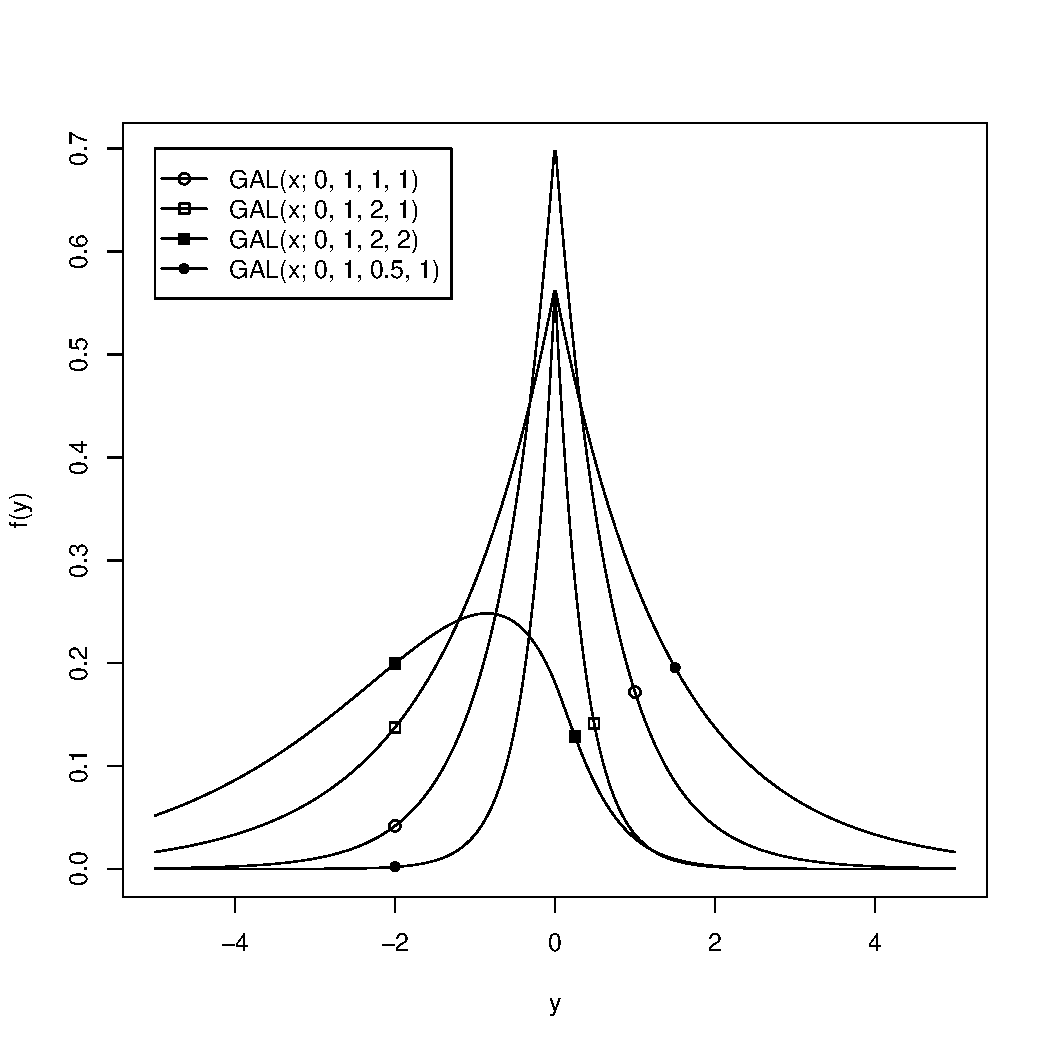
\includegraphics[scale=0.8]{./graphiques/dGAL-exemples.pdf}
  \caption{Fonction de densité de la distribution Laplace asymétrique
    généralisée avec différents paramètres:
    $GAL(y;\theta,\sigma,\kappa,\tau)$}
  \label{fig:densiteGAL}
\end{figure}

Afin de comparer la distribution de Laplace asymétrique généralisée
avec la normale, que l'on cherche à remplacer dans le contexte des
rendements financiers, le comportement des coefficients d'asymétrie
$\gamma_1$ et d'aplatissement $\gamma_2$ de celle-ci peut être
intéressant à observer. On obtient ces derniers à partir des moments
centraux \eqref{eq:momentsGAL} :
\begin{subequations}\label{eq:moments56GAL}
  \begin{align}
    \gamma_1(Y) &= \frac{m_3}{(m_2)^{3/2}} =
    \frac{2\,{\mu}^{3}+3\,{\sigma}^{2}\,\mu}{{\left( {\mu}^{2}+{\sigma}^{2}\right) }^{3/2}\,\sqrt{\tau}}\label{eq:moments5GAL}\\
    \gamma_2(Y) &= \frac{m_4}{(m_2)^{2}} - 3 = \frac{\left(
        3\,{\mu}^{4}+6\,{\sigma}^{2}\,{\mu}^{2}+3\,{\sigma}^{4}\right)
      \,{\tau}^{2}+\left(
        6\,{\mu}^{4}+12\,{\sigma}^{2}\,{\mu}^{2}+3\,{\sigma}^{4}\right)
      \,\tau}{{\left( {\mu}^{2}+{\sigma}^{2}\right) }^{2}\,{\tau}^{2}}
    - 3.\label{eq:moments6GAL}
  \end{align}
\end{subequations}

Le coefficient d'asymétrie de la normale vaut $\gamma_1^N(Y)=0$ et
celui d'excès d'aplatissement, $\gamma_2^N(Y)=0$, puisqu'il a été
défini à partir de cette distribution. Si l'on fixe tous les
paramètres sauf $\mu$, la valeur minimale du coefficient d'excès
d'aplatissement $\gamma_2(Y)$ est atteinte lorsque $\mu$ est de 0:
\begin{align*}
  \min_{\mu} \gamma_2(Y) &= \left[\gamma_2(Y)\right]_{\mu=0} \\
  &= \frac{3}{\tau}.
\end{align*}
Étant donné que le paramètre $\tau$ est strictement positif, la valeur
minimale que peut prendre le coefficient d'excès d'aplatissement
$\gamma_2(Y)$ est plus grande que 0. Par conséquent, l'aplatissement de la
distribution de Laplace asymétrique généralisée sera toujours
supérieur à celui de la normale; c'est donc une distribution
leptocurtique, ce qui est une propriété désirable selon les
observations de \cite{madan1990variance}.

\subsection{Changement d'échelle et de localisation}
\label{sec:transGAL}

Parfois, on doit modifier un ensemble de données afin d'effectuer des
comparaisons ou pour bénéficier des avantages d'une méthode
numérique. Les principales transformations utilisées sont:
\begin{enumerate}
\item un changement de localisation, où l'on additionne une constante
  à l'ensemble des données
\item un changement d'échelle, où l'on multiplie l'ensemble des
  données par un facteur
\item une combinaison des deux transformations précédentes.
\end{enumerate}

Soit deux constantes $a$, $b\neq0$ et une variable aléatoire $X$ qui
suit une distribution Laplace asymétrique généralisée: $X \sim
GAL(\theta,\sigma,\kappa,\tau)$. $Y$ correspond à la somme:
\begin{itemize}
\item de la constante $b$ et
\item du produit:
  \begin{itemize}
  \item de la constante $a$ et
  \item de la variable aléatoire $X$.
  \end{itemize}
\end{itemize}

Selon \cite{kotz2001laplace}, en utilisant le paramètre $\kappa$, on
peut effectuer un changement d'échelle et de localisation et obtenir
une variable aléatoire qui suit encore cette distribution:
\begin{itemize}
\item le paramètre de localisation $\theta$ subit la même
  transformation que la variable aléatoire $X$;
\item le paramètre d'échelle $\sigma$ est multiplié par la constante
  $a$;
\item le paramètre $\kappa$ est inversé si cette constante est
  négative. Ce dernier cas est en fait une réflexion de la
  distribution autour du mode.
\end{itemize}

On a donc:
\begin{align}
  \label{eq:GALscaletrans}
  Y = aX + b \sim GAL(a \theta + b,a\sigma,\kappa^{\sgn{a}\cdot
    1},\tau).
\end{align}

On estime les paramètres $\hat\theta, \hat\sigma, \hat\mu$ et
$\hat\tau$ sur un ensemble de données centrées et réduites $X_t$ à
partir d'un échantillon original $Y_t$. $\hat{m} \text{ et }
\hat{s}>0$ sont respectivement la moyenne et l'écart-type de
l'échantillon $Y_t$. En utilisant l'équation de transformation
\eqref{eq:GALscaletrans} avec les paramètres estimés précédemment, on
peut alors obtenir ceux correspondants pour l'échantillon:
\begin{align}
  \label{eq:transparamGALNS}
  Y_t = \hat{s} X_t + \hat{m} \sim GAL(\hat{s} \theta +
  \hat{m},\hat{s}\sigma,\kappa,\tau) .
\end{align}

Le paramètre $\kappa$ n'est pas modifié puisque l'écart-type $\hat{s}$
est strictement positif. Cette propriété permettra de pratiquer
l'estimation sur des données centrées et réduites, ce qui diminue le
risque d'erreurs numériques sans nuire à sa précision, puisqu'aucune
information contenue dans l'échantillon n'est perdue.

\subsection{Représentation alternative et simulation}
\label{sec:simulationGAL}

Le processus de Laplace $Y(t;\theta,\sigma,\kappa,\tau)$ peut être
représenté sous la forme d'une différence de deux processus gamma
$G_1(t;\tau) - G_2(t;\tau)$ à laquelle on additionne une composante de
dérive. Le premier processus compte les gains, alors que le second,
les pertes. Les deux ont des incréments qui suivent une distribution
gamma $\Gamma(\alpha=\tau, \beta=1)$, c'est-à-dire la même
distribution que le processus
subordonnant utilisé à la section \ref{sec:browniensub}:
\begin{align}
  \label{eq:distributiongammaformealt}
  G_i(\tau) \sim \Gamma\left(\tau,\beta=1 \right), \qquad i\in\left\{
    1,2 \right\}.
\end{align}

Il peut être représenté sous la forme du processus composé suivant:
\begin{align}
  \label{eq:processuslaplace2gamma}
  Y(t) \stackrel{d}{=} \theta +
  \frac{\sigma\sqrt{2}}{2}\left(\frac{1}{\kappa} G_1(t) - \kappa
    G_2(t)\right).
\end{align}

La distribution de Laplace asymétrique généralisée peut alors être
représentée sous la forme d'un incrément de ce processus. Les
variables aléatoires $G_1$ et $G_2$ sont respectivement des
réalisations indépendantes de distribution gamma avec densité
\eqref{eq:densitegamma1}:
\begin{align}
  \label{eq:differencegamma}
  Y \stackrel{d}{=} \theta + \frac{\sigma\sqrt{2}}{2} \left(
    \frac{1}{\kappa} G_1 - \kappa G_2 \right).
\end{align}

Simuler une réalisation de chacune d'entre elles suffira pour obtenir
une réalisation de la distribution gamma. On peut aussi réécrire la
définition précédente de la variable aléatoire $Y$
\eqref{eq:differencegamma} sous la forme simplifiée suivante:
\begin{align}
  \label{eq:differencegamma2}
  Y \stackrel{d}{=} \theta + \left(G_3-G_4 \right).
\end{align}

Les deux variables aléatoires sont alors définies comme suit:
\begin{align*}
  G_3 \sim \Gamma\left(\tau,\beta=\frac{\sqrt{2}}{\kappa\sigma} \right)\\
  G_4 \sim \Gamma\left(\tau,\beta=\frac{\kappa\sigma}{\sqrt{2}}
  \right).
\end{align*}

On peut facilement démontrer l'équivalence en distribution
\eqref{eq:differencegamma2}. En effectuant le produit des fonctions
caractéristiques respectives $\phi_{Y}(\xi)$, $\phi_{G_3}(\xi)$ et
$\phi_{G_4}(\xi)$ des variables aléatoires $Y$, $G_3$ et $G_4$, on
retrouve celle de la forme en $\kappa$:
\begin{align}
  \label{eq:equivalence2gammaFC}
  \phi_{Y}(\xi) &= e^{i\xi\theta} \cdot \phi_{G_3}(\xi) \cdot \phi_{G_4}(\xi) \nonumber\\
  &= e^{i\xi\theta} \cdot \left(\frac{1}{1+i\xi\cdot\frac{\kappa\sigma}{\sqrt{2}}}\right)^{\tau} \cdot \left(\frac{1}{1-i\xi\cdot\frac{\kappa\sigma}{\sqrt{2}}}\right)^{\tau} \nonumber\\
  &=
  \frac{e^{i\xi\theta}}{\left(1-i\xi\frac{\sigma}{\sqrt{2}}\left(\frac{1}{\kappa}-\kappa
      \right) + \frac{\sigma^2\xi^2}{2}\right)^{\tau}}.
\end{align}

La figure \ref{fig:simulGAL} présente un histogramme et un estimateur
de densité par noyau d'un échantillon de 2500 réalisations de la
variable aléatoire $Y$, suivant une distribution de Laplace
asymétrique généralisée de paramètres $\theta=0$, $\sigma=1$,
$\kappa=2$ et $\tau=1$. On remarquera que le paramètre $\kappa$
produit une distribution asymétrique à gauche puisqu'il prend une
valeur supérieure à 1.

\begin{figure}[!ht]
  \centering
  \includegraphics[scale=0.8]{"./graphiques/CH3-SIMULGAL0121"}
  \caption{Histogramme et estimateur de densité par noyau de 2500
    réalisations de la variable aléatoire $Y\sim
    GAL(\theta=0,\sigma=1,\kappa=2,\tau=1)$}
  \label{fig:simulGAL}
\end{figure}

\subsection{Fonction de Bessel et densité}
\label{sec:besseldensiteGAL}

La densité de la distribution Laplace asymétrique généralisée peut
être exprimée à l'aide de la fonction de Bessel modifiée du troisième
type \citep{abramowitz1965handbook}:
\begin{align}
  \label{eq:BesselK}
  K_{\lambda}(u) =
  \frac{(u/2)^{\lambda}\Gamma(1/2)}{\Gamma(\lambda+1/2)}
  \int_1^{\infty} e^{-ut} (t^2-1)^{\lambda-1/2}dt,\qquad \lambda \geq
  -1/2.
\end{align}

On définit les paramètres $\delta = \mu\sigma^{-1}$ et $\eta =
\sqrt{1+\delta^2}$ afin de simplifier la notation.  La démonstration
qui permet d'obtenir la fonction de densité est fondée sur la
définition de la distribution utilisant la différence de deux
processus gamma \eqref{eq:differencegamma}.  Elle est développée par
\cite{kozubowski1999class}:
\begin{align}
  \label{eq:densitekotz}
  f(x) &= \frac{e^{-\kappa^{\sgn(x)}|x|}}{\Gamma(\tau)} \int_{0}^{\infty} y^{\tau-1}(|x|+y)^{\tau-1}e^{-\eta y} dy \nonumber\\
  &= \frac{1}{\Gamma(\tau)\sqrt{\pi}} \left(\frac{|x|}{\eta}
  \right)^{\tau-1/2} e^{\delta x/2} K_{\tau-1/2}\left(\frac{\eta
      |x|}{2}\right).
\end{align}

Afin d'incorporer le paramètre de localisation $\theta$, on remplace
$x$ par la valeur centrée $x-\theta$, et les paramètres $\eta$ et
$\delta$ par ceux d'origine, tels que définis précédemment, pour
obtenir la forme suivante \citep{kotz2001laplace}:
\begin{align}
  \label{eq:densitekotz2001}
  f(x) =
  \frac{\sqrt{2}e^{\frac{\sqrt{2}}{2\sigma}(1/\kappa-\kappa)(x-\theta)}}{\sqrt{\pi}\sigma^{\tau+1/2}\Gamma(\tau)}
  \bigg(\frac{\sqrt{2}|x-\theta|}{\kappa+1/\kappa} \bigg)^{\tau-1/2}
  K_{\tau-1/2}\left(\frac{\sqrt{2}}{2\sigma}\left(\frac{1}{k}+\kappa
    \right)|x-\theta| \right).
\end{align}

Cette fonction a été implémentée dans un algorithme de maximum de
vraisemblance pour le logiciel GNU R par
\cite{RpackageVarianceGamma}. Elle reste cependant sensible
numériquement en plus de demander un temps de calcul important pour de
grands échantillons. De plus, comme la fonction de densité n'est pas
différentiable, on ne peut pas obtenir les estimateurs du maximum de
vraisemblance et leurs matrices de variance-covariance. Donc,
il est impossible d'effectuer de tests d'adéquation ou d'hypothèse avec ces
résultats. C'est une des principales raisons qui ont motivé la
recherche d'autres méthodes d'estimation plus efficaces pour cette
distribution.

\section{Cas particuliers}
\label{sec:cas-particuliers}

La distribution de Laplace asymétrique généralisée peut être
considérée comme une extension de plusieurs cas particuliers. Ces
distributions ainsi que leur notation et leur fonction de densité sont
présentées dans la table \ref{tab:casspeciauxGAL}.
\begin{table}[!ht]
  \centering
  \begin{tabular}{cccc}
    \hline
    \textbf{Cas} & \textbf{Distribution} & \textbf{Notation} & \textbf{Densité} \\
    \hline
    $\theta=0$ & \multirow{4}{*}{Exponentielle de moyenne $\mu>0$} & \multirow{4}{*}{$GAL(0,0,\mu,1)$} & \multirow{4}{*}{$\frac{1}{\mu}e^{-x/\mu}\,(x > 0)$} \\ 
    $\sigma=0$ &  &  &  \\
    $\mu>0$ &  &  &  \\ 
    $\tau=1$ &  &  &  \\ \hline
    $\theta=0$ & \multirow{3}{*}{Gamma de paramètres $\alpha=\tau$, $\beta=\mu>0$} &
    \multirow{3}{*}{$GAL(0,0,\mu,\tau)$} & \multirow{3}{*}{$\frac{x^{\tau-1}e^{-x/\mu}}{\mu^\tau\Gamma(\tau)},(x > 0)$} \\
    $\sigma=0$ &  &  &  \\
    $\mu>0$ &  &  &  \\ \hline
    $\sigma>0$ & \multirow{3}{*}{Laplace symétrique $(\sigma>0)$} &
    \multirow{3}{*}{$GAL(\theta,\sigma,0,1)$} & \multirow{3}{*}{$\frac{1}{\sqrt{2}\sigma}e^{-\sqrt{2}|x-\theta|/\sigma},(x \in \mathbb{R})$} \\
    $\mu=0$ &  &  &  \\
    $\tau=1$ &  &  &  \\ \hline
    $\sigma>0$ & \multirow{3}{*}{Laplace asymétrique $(\sigma>0)$} &
    \multirow{3}{*}{$GAL(\theta,\sigma,\mu,1)$} & \multirow{3}{*}{$\frac{\sqrt{2}\kappa}{\sigma(1+\kappa^2)}\begin{cases}e^{\frac{\sqrt{2}\kappa}{\sigma}(\theta-x)},\quad & x\geq\theta \\ e^{\frac{\sqrt{2}}{\sigma\kappa}(x-\theta)},\quad & x < \theta \end{cases}$} \\
    $\mu \neq 0$ &  &  &  \\
    $\tau=1$ &  &  &  \\ \hline
    $\sigma=0$ & \multirow{3}{*}{Dégénérée à $\theta$} & \multirow{3}{*}{$GAL(\theta,0,0,0)$} & \multirow{3}{*}{$1_{x=\theta}$} \\
    $\mu=0$ &  &  &  \\ 
    $\tau=0$ &  &  &  \\ \hline
  \end{tabular}
  \caption{Cas spéciaux de la distribution de Laplace asymétrique généralisée}
  \label{tab:casspeciauxGAL}
\end{table}

Les deux premiers cas spéciaux sont des distributions de probabilité
classiques. L’attention sera portée sur la distribution de Laplace
asymétrique et son cas spécial, celle de Laplace symétrique. La
dégénérée n'a aucune application pratique, mais en mentionner
l'existence est pertinent, puisque ce ne sont pas toutes les
distributions qui admettent ce cas.

\subsection{Distribution de Laplace asymétrique}
\label{sec:distributionAL}

La distribution de Laplace asymétrique a été introduite
par \cite{hinkley1977estimation} et étudiée en profondeur par
\cite{kozubowski1999class}.  Cette distribution a elle aussi plusieurs
caractéristiques intéressantes pour remplacer la normale, dans le
contexte de la modélisation financière, comme le présentent
\cite{kozubowski2001asymmetric}. Elle est notée
$AL(\theta,\sigma,\kappa)$.

Cette distribution, en tant que cas particulier de la distribution de
Laplace asymétrique généralisée, conserve la majorité de ses
propriétés.  Entre autres, elle est infiniment divisible et possède des moments
finis. Les paramètres $\theta$, $\sigma$ et $\kappa$ conservent leurs
rôles et propriétés définis à la section \ref{sec:momentsGAL}. On peut
donc contrôler la localisation, l'échelle et l'asymétrie de la
distribution. Cependant, aucun paramètre ne permet de contrôler le
coefficient d'aplatissement.

La densité de probabilité de cette distribution
$f(x;\theta,\sigma,\kappa)$ présente une forme analytique simple qui
ne requiert pas le recours à la fonction de Bessel modifiée de
troisième type \eqref{eq:BesselK}.
\begin{align}
  \label{eq:densiteAL}
  f(x;\theta,\sigma,\kappa) =
  \frac{\sqrt{2}}{\sigma}\frac{\kappa}{1+\kappa^2} \begin{cases}
    \exp\left(\frac{-\sqrt{2}\kappa}{\sigma}\left( x-\theta \right)\right),\quad & x\geq\theta \\
    \exp\left( \frac{\sqrt{2}}{\theta\kappa}\left(\theta - x \right)
    \right),\quad & x<\theta.\end{cases}
\end{align}

La fonction caractéristique de cette distribution prend la forme
suivante:
\begin{align}
  \label{eq:caractALkappa}
  \phi(t;\theta,\sigma,\kappa) = \frac{e^{i \theta
      t}}{1+\frac{\sigma^2 t^2}{2}-
    i\frac{\sigma}{\sqrt{2}}\left(\frac{1}{\kappa}-\kappa \right)
    t}\,.
\end{align}

Cette dernière est utilisée principalement lorsque l'application d'une
propriété nécessite une distribution avec un seul paramètre d'échelle.
La seconde paramétrisation de cette distribution utilise le paramètre
$\mu$ qui n'est pas invariant d'échelle.  Cette paramétrisation donne
une forme beaucoup plus simple de la fonction caractéristique
\eqref{eq:caractALkappa}:
\begin{align}
  \label{eq:caractALmu}
  \phi(t\theta,\sigma,\mu) = \frac{e^{i \theta t}}{1+\frac{\sigma^2
      t^2}{2}- i\mu t}.
\end{align}

On reconnait la fonction caractéristique d'un incrément du processus
de Laplace \eqref{eq:fncaractprocessuslaplace} avec les paramètres
($\tau=1$, $t=1$). Une forme standardisée de cette distribution existe
aussi avec le paramètre d'échelle $\sigma=1$ et de dérive $\theta=0$.
Enfin, on peut avoir une représentation alternative de cette
distribution, utilisée principalement pour la simulation, basée sur
l'exponentielle:
\begin{align}
  \label{eq:ALrepsimul}
  Y &= \theta + \frac{\sigma}{\sqrt{2}} \left(\frac{1}{\kappa}W_1 - k W_2 \right)
\end{align}
où
\begin{align*}
  W_1 \sim \mbox{Exponentielle}\left(\frac{\sigma}{\sqrt{2}\kappa}\right) \nonumber \mbox{ et } W_2 \sim \mbox{Exponentielle}\left(\frac{\sigma\kappa}{\sqrt{2}}\right)
\end{align*}

Cette méthode n'est cependant pas la plus efficace pour simuler une
réalisation $Y$ de la distribution de Laplace asymétrique, car on peut
la faire à partir de deux réalisations indépendantes $U_1$ et $U_2 $
d'une variable aléatoire uniforme définie sur l'intervalle
$\left[0,1\right]$:
\begin{align}
  \label{eq:simulALunif}
  Y = \theta + \frac{\sigma}{\sqrt{2}}
  \ln{\frac{U_1^\kappa}{U_2^{1/\kappa}}}.
\end{align}

Lorsque le paramètre $\tau$ de la distribution de Laplace asymétrique
généralisée est un entier, on peut générer une réalisation $X$ de
celle-ci en sommant un total de $\tau$ réalisations indépendantes de
la variable aléatoire $Y$:
\begin{align*}
  X &= \sum_{i=1}^{\tau} Y_{i} \\
  Y_{i} &\sim AL(\theta,\sigma,\kappa).
\end{align*}

\section{Relation avec le modèle de \cite{madan1990variance}}
\label{sec:relation-avec-le}

Le modèle Variance Gamma de \cite{madan1990variance} utilise une
paramétrisation différente de celle de \cite{kotz2001laplace}. On
doit, afin de conserver une compatibilité des développements des
prochains chapitres, détailler les changements de paramètres qui
permettent de passer d'un modèle à l'autre. Le modèle Variance Gamma
utilise les paramètres $C,\sigma,\theta \mbox{ et } \nu$. Afin
d'éviter la confusion, les paramètres seront indicés de 1 à 3 selon le
modèle d'où ils proviennent. Le modèle 1 sera celui de
\cite{madan1990variance}, les modèles 2 et 3 seront respectivement les
paramétrisations en $\mu$ et en $\kappa$ de
\cite{kotz2001laplace}. Les différentes équivalences se trouvent à la
table \ref{tab:chparam}.
\begin{table}[!ht]
  \centering
  \begin{tabular}{cccccc}
    \hline
    \textbf{Vers le modèle} & &  & \textbf{À partir du modèle} &  & \textbf{À partir du modèle} \\ \hline
    \textbf{1} & &  & \textbf{2} &  & \textbf{3} \\ \hline
    
    & $C$ & $=$ & $\theta_2$ & $=$ & $\theta_3$ \\ 
    \multicolumn{ 1}{l}{} & $\sigma_1$ & $=$ & $\sqrt{\tau_2}\sigma_2$ & $=$ & $\sqrt{\tau_3}\sigma_3$ \\ 
    \multicolumn{ 1}{l}{} & $\theta_1$ & $=$ & $\mu\tau_2$ & $=$ & $\tau_3\sigma_3(1/\kappa - \kappa)/\sqrt{2}$ \\ 
    \multicolumn{ 1}{l}{} & $\nu$ & $=$ & $1/\tau_2$ & $=$ & $1/\tau_3$ \\ 
    \hline
    \textbf{2} & &  & \textbf{1} &  & \textbf{3} \\ \hline
    & $\theta_2$ & $=$ & $C$ & $=$ & $\theta_3$ \\ 
    \multicolumn{ 1}{l}{} & $\sigma_2$ & $=$ & $\sigma_1\sqrt{\nu}$ & $=$ & $\sigma_3$ \\ 
    \multicolumn{ 1}{l}{} & $\mu$ & $=$ & $\theta_1*\nu$ & $=$ & $\sigma_3(1/\kappa - \kappa)/\sqrt{2}$ \\ 
    \multicolumn{ 1}{l}{} & $\tau_2$ & $=$ & $1/\nu$ & $=$ & $\tau_3$ \\ 
    \hline
    \textbf{3} & &  & \textbf{1} &  & \textbf{2} \\ \hline
    & $\theta_3$ & $=$ & $C$ & $=$ & $\theta_2$ \\ 
    \multicolumn{ 1}{l}{} & $\sigma_3$ & $=$ & $\sigma_1\sqrt{\nu}$ & $=$ & $\sigma_2$ \\ 
    \multicolumn{ 1}{l}{} & $\kappa$ & $=$ & $\frac{\sqrt{2(\sigma_1\sqrt{\nu})^2 + (\theta_1*\nu)^2} – \theta_1*\nu}{\sigma_1\sqrt{\nu}\sqrt{2}}$ & $=$ & $\frac{\sqrt{2(\sigma_2)^2 + \mu^2} - \mu}{\sigma_2\sqrt{2}}$ \\ 
    \multicolumn{ 1}{l}{} & $\tau_3$ & $=$ & $1/\nu$ & $=$ & $\tau_2$ \\ \hline
  \end{tabular}
  \caption{Changements de paramétrisation}
  \label{tab:chparam}
\end{table}



%%% Local Variables: 
%%% mode: latex
%%% TeX-master: "gabarit-maitrise"
%%% End: 

